\section{Differentitaion}
\label{sec:differentiation}
To chacarcterize the influence of \ac{pdgf} on \acp{haomc}, the cells were first treated with \ac{tgf} for two days to push them from a probably dedifferentiated phenotype during cultivation and lack of stimulation towards one that resambles the contractile phenotpye as a standardized starting point. Further cells were stimulated for four days with \ac{il1} and \ac{pdgf}. The induced phenptypes were then characterized via \ac{qpcr} and Seahorse Assay.

    \subsection{Expression of CNN1 \& MMP9}
    \label{subsec:qPCR}
    \begin{figure}[h!]
    \capstart
        \centering
    	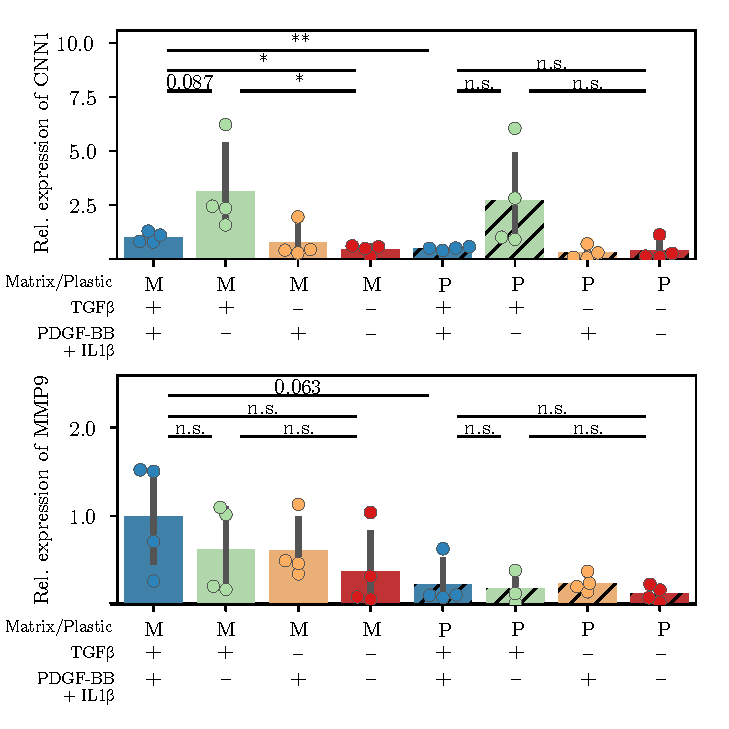
\includegraphics{Abbildung/qPCR.pdf}

    	\begin{minipage}{\captionwidth}
    		\caption[CNN_qPCR]{\uzlemph{Relative Expression of \ac{cnn1} \& \ac{mmp9} in \acp{haosmc}} \newline qPCR analysis of expression for contractile marker \ac{cnn1} (top) and synthetic marker \ac{mmp9} (bottom) for \acp{haosmc} differentiated with different combinations of cytokines:
            \textbf{++:} 2 d with \ac{tgf} followed by 4 d with \ac{il1} \& \ac{pdgf};
            \textbf{+–:} 2 d with \ac{tgf} followed by 4 d without stimulation;
            \textbf{–+:} 2 d without stimulation followed by 4 d with \ac{il1} \& \ac{pdgf};
            \textbf{––:} 6 d without stimulation.
            All four conditions were tested on two differen surfaces (plastic vs. \ac{col1} matrix). Expression levels are in relation to expression of housekeeping gene \ac{gapdh}. Statistical analysis for (n = 4) biological repeats was performed using student's T-test: $*: p < 0.05; **: p < 0.01$}
    		\label{fig:qPCR}
    	\end{minipage}
    \end{figure}

    To track the differentatiation and confirm that the \acp{haosmc} first adopt a chontractile phenotype after \ac{tgf} stimulation and then further dedifferentiate after stimulation with \ac{pdgf}, the mRNA levels of the marker genes \ac{cnn1} as well as \ac{mmp9} were determined using \ac{qpcr}. \ac{cnn1} as a contractivle marker and \ac{mmp9} as a marker for a synthetic phenotype. For better compariability mRNA levels are considered in realtion to the house keeping gene \ac{gapdh}.

    As seen in figure \ref{fig:qPCR} (top panel), stimulation of \acp{haosmc} cultivated on a \ac{col1}-Matrix with \ac{tgf} causes a significant increase in \ac{cnn1} expression (+– vs. – –). After further stimulation with \ac{pdgf} \& \ac{il1}, while not significant, \ac{cnn} expression declines again (+– vs. ++) but is still significantly higher than in \acp{haosmc} which were not stimulated at all (– – vs. ++). A similar trend seems to take place for \acp{haosmc} cultivated on plastic, while not significant with four biological repeats repeats. Further stimulation of \acp{haosmc} on plastic with \ac{tgf} followed by stimulation with \ac{pdgf} \& \ac{il1}, yields a significantly higher expression of \ac{cnn1} (++ Matrix vs. ++ Plastic).

    As seen in the bottom panel of figure \ref{fig:qPCR}, within 4 biological repeats, no statistically significant trends can be observed for the expression of \ac{mmp9}. Still the avarage expression of \ac{mmp9} seems to approx. doubled for all conditions, the most prominent difference being between \acp{haosmc} treated first with \ac{tgf}, then with \ac{pdgf} \& \ac{il1} (++ Matrix vs. ++ Plastic, p = 0.063).


    \subsection{Energy profile}
    \label{subsec:energy}
    In additition to the expression of \ac{cnn1} \& \ac{mmp9}, the energy profiles of \acp{haosmc} were assesed via Seahorse Assay. It is important to note, that the assay was carried out on plastic because the \ac{col1} matrix does not fit into the confined compartment created by the pistion for detection of \ac{ocr} \& \ac{ecar}. Further only two biological repeats were carried out, because it became increasingly clear, that all other experiments would be cariied out on a \ac{col1}. Therefore all following results should be considered under these circumstances.

    \begin{figure}[h!]
    \capstart
        \centering
        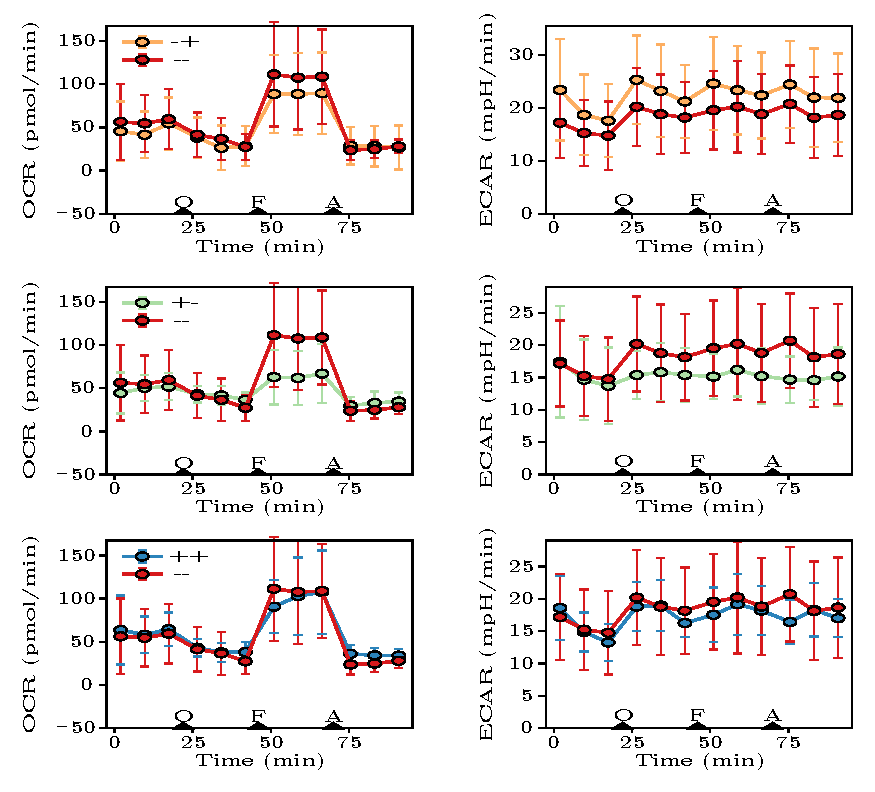
\includegraphics{Abbildung/Seahorse_tracks.pdf}

        \begin{minipage}{\captionwidth}
            \caption[seahorse_tracks]{\uzlemph{\ac{ocr} \& \ac{ecar} of \acp{haosmc}} \newline Seahorse assay for \acp{haosmc} differentiated with different combinations of cytokines.
            \textbf{++:} 2 d with \ac{tgf} followed by 4 d with \ac{il1} \& \ac{pdgf};
            \textbf{+–:} 2 d with \ac{tgf} followed by 4 d without stimulation;
            \textbf{–+:} 2 d without stimulation followed by 4 d with \ac{il1} \& \ac{pdgf};
            \textbf{––:} 6 d without stimulation.
            \ac{ocr} \& \ac{ecar} are shown for –+ (top), +– (middle) and ++ (bottom) in comparison to ––. Injectiontimes for toxins (O: Oligomycin; F: FCCP; A: Antimycin A) are marked as triangles. All tracks were recorded for cells cultivated on plastic. Shown datapoints are the average of (n = 2) biological repeats.
            }
            \label{fig:seahorse_tracks}
        \end{minipage}
    \end{figure}

    The readout paramters of the Seahorse assay are \ac{ocr} as a representation of mitochondrial activity and the \ac{ecar}, representing glycolytic activity of the cells. \ac{ocr} and \ac{ecar} for \acp{haosmc} displayed in figure \ref{fig:seahorse_tracks}. All cells show characteristic changes in \ac{ocr} after addition of toxins impacting the respiratory chain (compare to figure \ref{fig:seahorse_basics} B). After inhibition of the ATP synthase with with Oligomycin, the basal \ac{ocr} drops, this way making the proportion of the \ac{ocr} accessible that was required for \ac{atp} production. Further addition of \ac{fccp} decouples the respiratory chain, destroying the proton gradiant over the mitochondiral membran and letting the cells reach their maximal respiratory capacity. Finally, the inhibition of coenzyme Q-cytochrome c reductase (complex III) with Antimycin A, stops all mitochondrial respiratory activity. The \ac{ecar} shows a mild increase after addition of Oligionmycin, most likely because the cells are compensating the loss of mitochondiral \ac{atp} production via increased glycolysis.

    \begin{figure}[h!]
    \capstart
        \centering
    	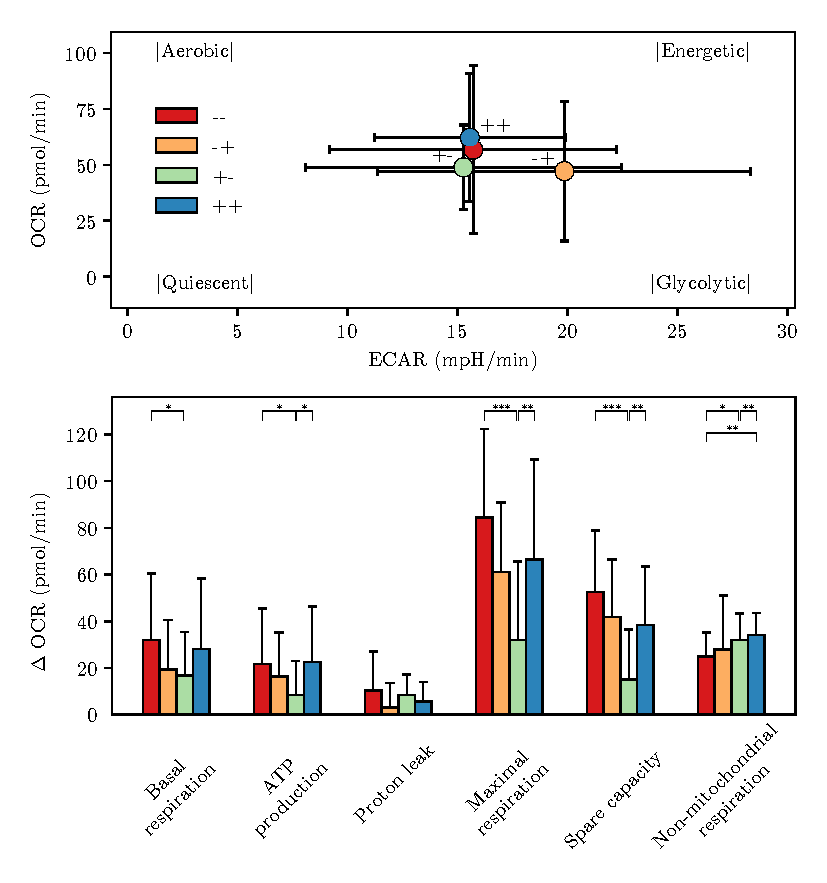
\includegraphics{Abbildung/Seahorse_summary_merged.pdf}

    	\begin{minipage}{\captionwidth}
    		\caption[energy_profile]{\uzlemph{Energy profile of \acp{haosmc}} \newline Seahorse assay for \acp{haosmc} differentiated with different combinations of cytokines as described in figure \ref{fig:seahorse_tracks}.
            (\textbf{A}) Initial \ac{ocr} \& \ac{ecar} of the four tested conditions. (\textbf{B}) Characteristics of the the respiratory chain calculated from the tracks shown in figure \ref{fig:seahorse_tracks} as described in section \ref{sec:methods_seahorse}. Statistical analysis for (n = 2) biological repeats was performed using student's T-test: $*: p < 0.05; **: p < 0.01, ; ***: p < 0.001$}
    		\label{fig:energy_profile}
    	\end{minipage}
    \end{figure}

    Looking at the energy profile of the \acp{haosmc} it is easy to see that \ac{ocr} \& \ac{ecar} are quite similar for the conditions ++, +– and ––. The only outlier showing a higher \ac{ecar}, are \acp{haosmc} only stimulated with \ac{il1} \& \ac{pdgf} (fig. \ref{fig:energy_profile}, A). More interesting difference can be observed when examining characterics of the respiratory chain. Stimulation with only \ac{tgf} causes a sigbnificant decrease in basal respiration, \ac{atp} production, maximal respiration as well as spare capacity (figure \ref{fig:energy_profile}, B top). Further stimulation with \ac{il1} \& \ac{pdgf} then causes again significant increase of these paramters to similar levels as in undifferentiated \acp{haosmc} (figure \ref{fig:energy_profile}, B bottom).

\section{Evaluation of oxidative Stress}
\label{sec:oxStress}
Finally it was evaluated if further stimulation with \ac{pdgf} would yield generation of \ac{ros} to an extend that can not be compensated by the \ac{ros} defense and lead to oxidative stress.

    \subsection{PDGF boost of out cells indcues oxidative stress}

    \begin{figure}[h!]
    \capstart
        \centering
    	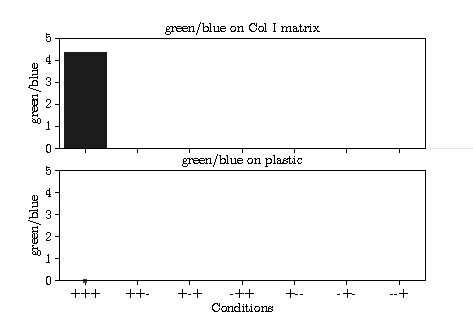
\includegraphics{Abbildung/CellROX_initial_cond.pdf}

    	\begin{minipage}{\captionwidth}
    		\caption[repeat_Lisa]{\uzlemph{Boost with \ac{pdgf} induces generation of \ac{ros}.} \newline CellROX assay for \acp{haosmc} differentiated with different combinations of cytokines: 2 d with \ac{tgf}; followed by 4 d with \ac{il1} \& \ac{pdgf}; follwoed by 2 h boost with 200 ng/mL \ac{pdgf}. Differentiation and assay carried out on \ac{col1} matrix (top) or plastic (bottom). Shown signal was calculated according to section \ref{subsec:cellrox_data_processing} as the CellROX Green signal, normalized by DAPI signal. No statistica analysis for (n = 1) biological repeats was performed. }
    		\label{fig:cellrox_8con}
    	\end{minipage}
    \end{figure}

    At first an experiment already done in the group was repeated. Stimulating the four tested combinations of + 5 ng/mL \ac{tgf} as well as 10 ng/mL  \ac{il1} \& 10 ng/mL  \ac{pdgf} stimulated cells, for two more hours with 200 ng/mL As displayed in figure \ac{pdgf} in \ac{hbss}. As displayed in figure \ref{fig:cellrox_8con} only stimulation for two days with \ac{tgf}, followed by 2 days with \ac{il1} \& \ac{pdgf}, followed by 2 h boost with \ac{pdgf} was able to trigger noticable generation of \ac{ros}.

    \subsection{Characterization of the CellROX Assay}
    \begin{figure}[h!]
    \capstart
        \centering
    	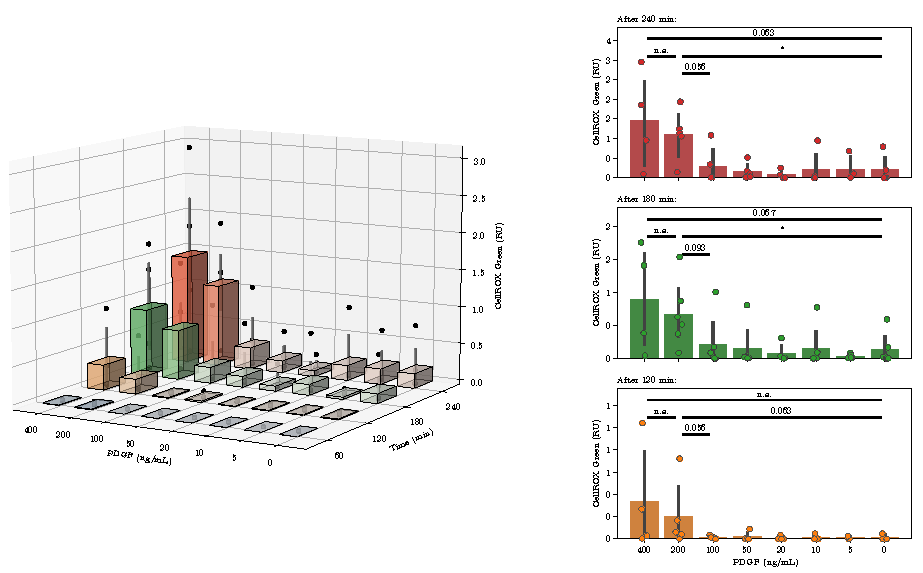
\includegraphics{Abbildung/CellROX_titration_no_norm.pdf}

    	\begin{minipage}{\captionwidth}
    		\caption[cellROX_titration]{\uzlemph{\ac{pdgf} boost titration} \newline
            CellROX assay for \acp{haosmc} differentiated with different combinations of cytokines: 2 d with \ac{tgf}; followed by 4 d with \ac{il1} \& \ac{pdgf}; follwoed by 4 h boost with 0 - 400 ng/mL \ac{pdgf}. Differentiation and assay carried out on \ac{col1} matrix.
            (\textbf{A}) 3D visualization: CellROX green signal as a function of \ac{pdgf} concnentration during the boost as well as incubation time.
            (\textbf{B}) 2D visualization: CellROX green signal as a function of \ac{pdgf} concnentration after 120 min, 180 min \& 240 min.
            Shown signal was calculated according to section \ref{subsec:cellrox_data_processing} as the CellROX Green signal, normalized by DAPI signal. Statistical analysis for (n = 6) biological repeats was performed using Mann-Whitney U test: $*: p < 0.05; **: p < 0.01$. It is important to note that not for every biological repeat \textit{all} \ac{pdgf} concentration were tested. }
    		\label{fig:cellROX_titration}
    	\end{minipage}
    \end{figure}

    To get a better understanding of the assay and its limits a titration was carried out. For this \acp{haosmc} stimulated for 2 d with 5 ng/mL \ac{tgf} as well as 4 d with 10 ng/mL  \ac{il1} \& 10 ng/mL  \ac{pdgf}, were boosted with different concentrations of \ac{pdgf} (0 - 400 ng/mL). Signal was detected after 60, 120, 180 \& 240 minutes in \ac{hbss}. As seen in figure \ref{fig:cellROX_titration}, CellROX Green signal is neglable after 60 min and then increases with elongated boost times. Further CellROX Green signal stays negalble for boost concentrations 100 ng/mL \ac{pdgf}. Signal is significantly higher for boost with 200 ng/mL \ac{pdgf} than it is for no boost after 180 min (figure \ref{fig:cellROX_titration} B middle) and 240 min (figure \ref{fig:cellROX_titration} B top). While signal in wells boosted with 400 ng/mL \ac{pdgf} was further increased in regard to boost with 200 ng/mL \ac{pdgf} in two cases, the signal also collapsed in two repeats. For this reason the avarage signal for boost with 400 ng/mL \ac{pdgf} is the highest but the increase is not statistically significant.

    \begin{figure}[h!]
    \capstart
        \centering
    	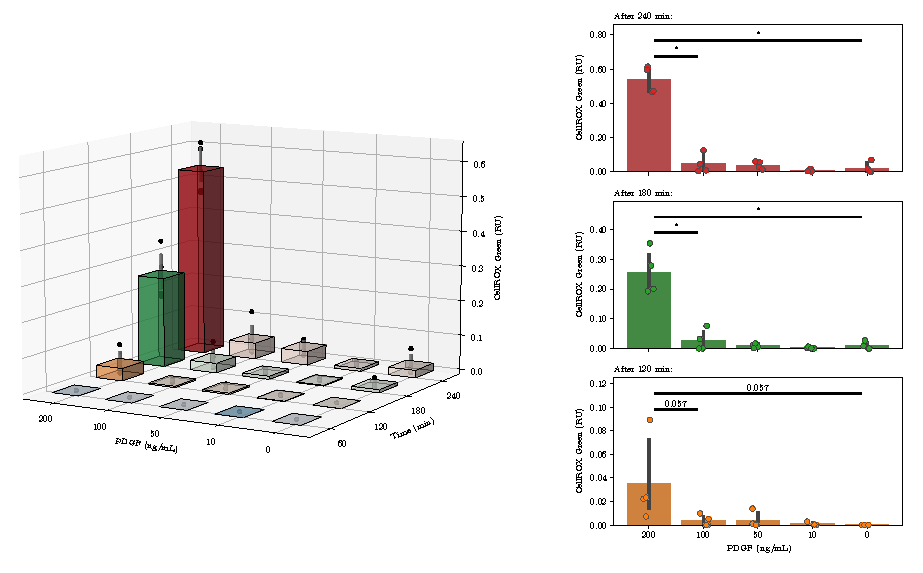
\includegraphics{Abbildung/CellROX_titration_norm.pdf}
    	\begin{minipage}{\captionwidth}
    		\caption[cellROX_titration_norm]{\uzlemph{\ac{pdgf} boost titration - normalized} \newline
            CellROX assay for \acp{haosmc} differentiated with different combinations of cytokines: 2 d with \ac{tgf}; followed by 4 d with \ac{il1} \& \ac{pdgf}; follwoed by 4 h boost with 0 - 200 ng/mL \ac{pdgf}. Differentiation and assay carried out on \ac{col1} matrix.
            (\textbf{A}) 3D visualization: CellROX green signal as a function of \ac{pdgf} concnentration during the boost as well as incubation time.
            (\textbf{B}) 2D visualization: CellROX green signal as a function of \ac{pdgf} concnentration after 120 min, 180 min \& 240 min.
            Shown signal was calculated according to section \ref{subsec:cellrox_data_processing} as the CellROX Green signal, normalized by DAPI signal, further the signal was normalized via the total signal of the biological repeat. Statistical analysis for (n = 4) biological repeats was performed using Mann-Whitney U test: $*: p < 0.05; **: p < 0.01$.}
    		\label{fig:cellROX_titration_norm}
    	\end{minipage}
    \end{figure}

    Overall the trend of greatly increased CellROX signal for boost with 100 as well as 200 ng/mL \ac{pdgf} was consistent within biological repeats, however variance between repeats was almostas high as differences between the conditions. Potential causes for this phenomenon are discussed in section \ref{link to diskussion when I write it}. To account for this large variation between biological repeats, the assay was reevaluated by selection of shared conditions among four biological repeats and normalized by the cummulative intensity of all conditions of the biological repeat (see figure \ref{fig:cellROX_titration_norm}). This way compensating for differences between biological repeats and resulting in the same observation as without normalization. CellROX signal after 180 min or 240 is signalifcantly higher for cells boostes with \ac{pdgf} than cell that were not boosted (0 ng/mL \ac{pdgf}).

    \subsection{Rescue of ROS production using NAC}
        \begin{figure}[h!]
    \capstart
        \centering
    	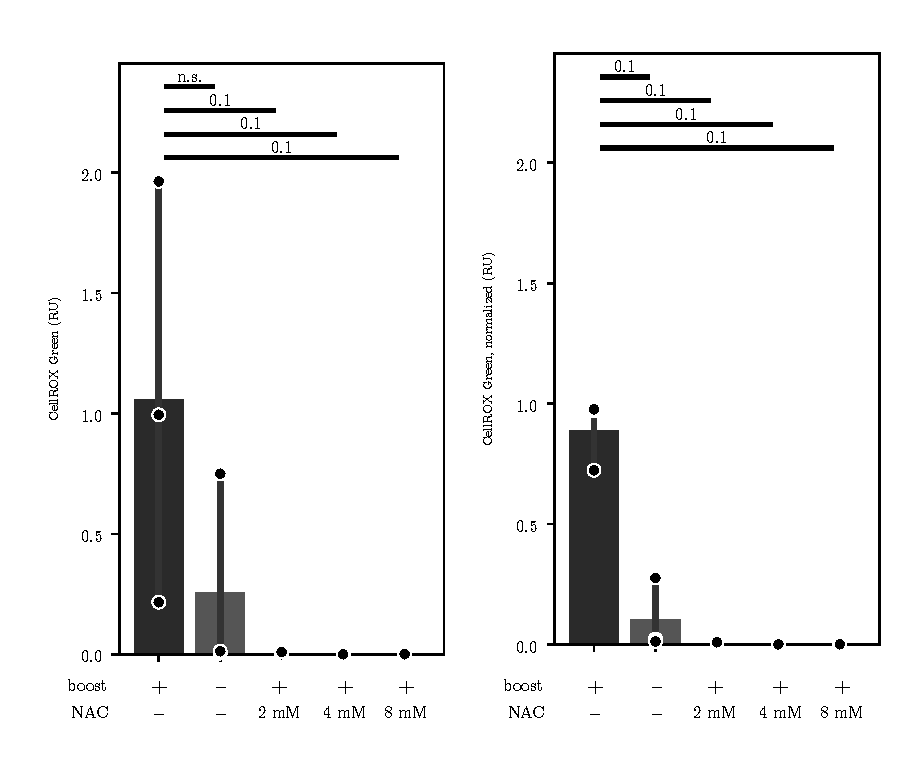
\includegraphics{Abbildung/NAC_quench.pdf}

    	\begin{minipage}{\captionwidth}
    		\caption[NAC quench]{\uzlemph{\ac{ros} generation due to \ac{pdgf} boost can be rescued with \ac{nac}} \newline
            CellROX assay for \acp{haosmc} differentiated with different combinations of cytokines: 2 d with \ac{tgf}; followed by 4 d with \ac{il1} \& \ac{pdgf}; follwoed by 3 h boost with 200 ng/mL \ac{pdgf}. Differentiation and assay carried out on \ac{col1} matrix. Cells were treated with 2, 4, or 8 mM of \ac{nac} 2 h before the assay.
            Shown signal was calculated according to section \ref{subsec:cellrox_data_processing} as the CellROX Green signal, normalized by DAPI signal (\textbf{A}), further the signal was normalized via the total signal of the biological repeat (\textbf{B}). Statistical analysis for (n = 4) biological repeats was performed using Mann-Whitney U test: $*: p < 0.05; **: p < 0.01$.
            pos Ctrl: not treated with \ac{nac}, negCtrl: no boost with \ac{pdgf}}
    		\label{fig:NAC_quench}
    	\end{minipage}
    \end{figure}

    Finally, a rescue experiment was performed, to verify that observed signal in the CellROX assay was indeed due to generation of \ac{ros}. For this \ac{ros} generation was quenched by the addition of 2, 4, or 8 mM of \ac{nac}. Indeed (while not statistically significant) a clear trend can be observed, that \acp{haosmc} treated with \ac{nac} shows no signal.
    In the end, it should be noted, that the signal onyl build up over 15 - 20 minutes under the microscope after the cells were taken out of the incubator. This indicates that generateion of \ac{ros} might not exclusively triggered by \ac{pdgf} stimulation but also required additional contributors like the loss the optimized atmosphere of 37°C and 5 \% CO2 in the incubator. This might not have been noted during the titration assay, because cells were taken out of the incubator after one hour anyway to image them for the first time.

\section{Database and GWAS Visualizer}
This was quite a long process, tinkering around with different designs to get a working solution. For this use case visualization in the browser using a database as the backend was the final decision. Compare to fetching everything online -> slow and just grabbing everything from files -> extremely stressful to maintain.

    \subsection{Curation of Data}
    Describe what actually happend to the data, probably in the methods section.
    This should be pretty self explanatory. Just have a look at the table and figure.

    \begin{table}[h!]
    \capstart
    \centering
    \begin{minipage}{\captionwidth}
        \caption[db tables]{\uzlemph{List of Database Tables}\newline
        List of all the datasets and corresponding tables which were funneled into the database. The size of the tables (and accompanying indices) is indicated by the number of databank pages that are reserved for the data, each page fitting 4096 bytes.}
        \label{tab:db_tables}
    \end{minipage}
        \begin{tabular}{l|l|l}
        Data                                       & Tables                             & Page count (including indices)                                                                      \\ \hline
        \multirow{3}{*}{GWAS Summary stats}        & variation                          & 418318                                                                                              \\
                                                   & gwas\_meta\_cad                    & 867025                                                                                              \\
                                                   & identified\_proxy\_SNPs\_tbl       & 4                                                                                                   \\ \hline
        \multirow{2}{*}{HGNC gene list}            & hgnc\_all\_symbols\_tbl            & 826                                                                                                 \\
                                                   & hgnc\_approved\_symbols\_tbl       & 592                                                                                                 \\ \hline
        \multirow{3}{*}{Linked SNPs}               & linked\_SNPs\_tbl                  & 8819                                                                                                \\
                                                   & population\_tbl                    & 1                                                                                                   \\
                                                   & consequence\_tbl                   & 1                                                                                                   \\ \hline
        \multirow{2}{*}{Ensembl Genome Annotation} & ensembl\_genelist\_tbl             & 613                                                                                                 \\
                                                   & ensembl\_genelist\_biotypes\_tbl   & 1                                                                                                   \\ \hline
        \multirow{2}{*}{Ensembl Regulatory Build}  & ensembl\_reg\_build\_tbl           & 8778                                                                                                \\
                                                   & ensembl\_reg\_build\_features\_tbl & 1                                                                                                   \\ \hline
        TSS                                        & tss\_tbl                           & 481                                                                                                 \\ \hline
        Open Target Genetics Scores                & opentarget\_l2g\_tbl               & 40984                                                                                               \\ \hline
        \multirow{2}{*}{GWAS catalog}              & gwascatalog\_associations\_tbl     & 10569                                                                                               \\
                                                   & gwascatalog\_studies\_tbl          & 326                                                                                                 \\ \hline
        \multirow{2}{*}{TADs}                      & tad\_tbl                           & 902                                                                                                 \\
                                                   & tad\_sample\_tbl                   & 1                                                                                                   \\ \hline
        \multirow{2}{*}{scATAC seq textcite\{\}}   & clint\_miller\_tbl                 & 12370                                                                                               \\
                                                   & clint\_miller\_biotypes\_tbl       & 1                                                                                                   \\ \hline
        \multirow{2}{*}{scATAC seq CATlas}         & catlas\_tbl                        & 308574                                                                                              \\
                                                   & catlas\_biotypes\_tbl              & 3                                                                                                   \\ \hline
        \multirow{4}{*}{ABC model}                 & abc\_tbl                           & 153920                                                                                              \\
                                                   & abc\_targetgenes\_tbl              & 84                                                                                                  \\
                                                   & abc\_celltypes\_tbl                & 3                                                                                                   \\
                                                   & abc\_classes\_tbl                  & 1                                                                                                   \\ \hline
        \multirow{2}{*}{ENCODE cCREs}              & ENCODE\_CCRE                       & 4451476                                                                                             \\
                                                   & ENCODE\_CCRE\_META                 & 107                                                                                                 \\ \hline
        total                                      & -                                  & 6284781 ($\approx$ 25.75 GB)
        \end{tabular}
    \end{table}

    \begin{figure}[h!]
    \capstart
        \centering
        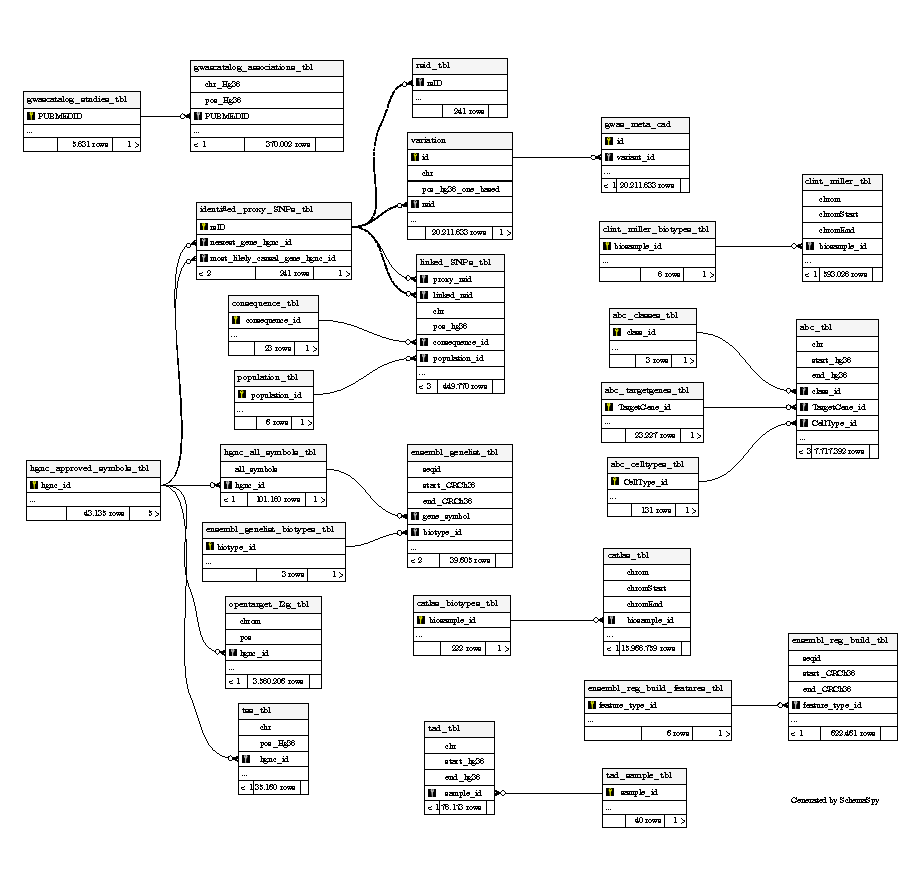
\includegraphics{Abbildung/db-schema.pdf}

        \begin{minipage}{\captionwidth}
            \caption[database]{\uzlemph{Entity-Relationship Diagram of the Database}\newline
            Fields and relationships of the tables listed in table \ref{tab:db_tables}. The diagram was generated via SchemaSpy.}
            \label{fig:db_er}
        \end{minipage}
    \end{figure}



    \subsection{Visualization}
    \label{subsec:result_vis}
    Building on the initially intended use case for the data a visualization tool was build as briefly described in the methods section, for more details please check the source code or just ask.

    Describe what the tool can do. Search function for SNPs, also for genes, providing info for associated SNPs. Visualization of the window SNPs, including linked SNPs annotated with important info such as most severe consequence. Further the data is aligned with important stuff like overlapping genes (integrating l2g scores). Also enesembl regulatory build and TADs. Further a lot of cell specific data in the form of scATAC seq tracks and promotor gene links from the ABC model. These are also shown and for easier navigation grouped into different classes using cellosaurus. To have a better look a individual variants these can be clicked, only highlighting tracks that overlap with the specific selected variant.

    For more information regarding the aligned data please check the corresping paragraph in the intrdocution.

\section{Enrichment analysis}
\label{sec:result_enrichment}
The only data that is not displayed in the plot are cCRE elements which were used for an enrichment analysis. Checking different biosamples for significant enrichment of \acp{ccre} that are overlapping with proxy SNPs identified in the \ac{cad} \ac{gwas} or variants that are in \ac{ld} with these. The procedure is described described in methods.

\begin{figure}[h!]
\capstart
    \centering
	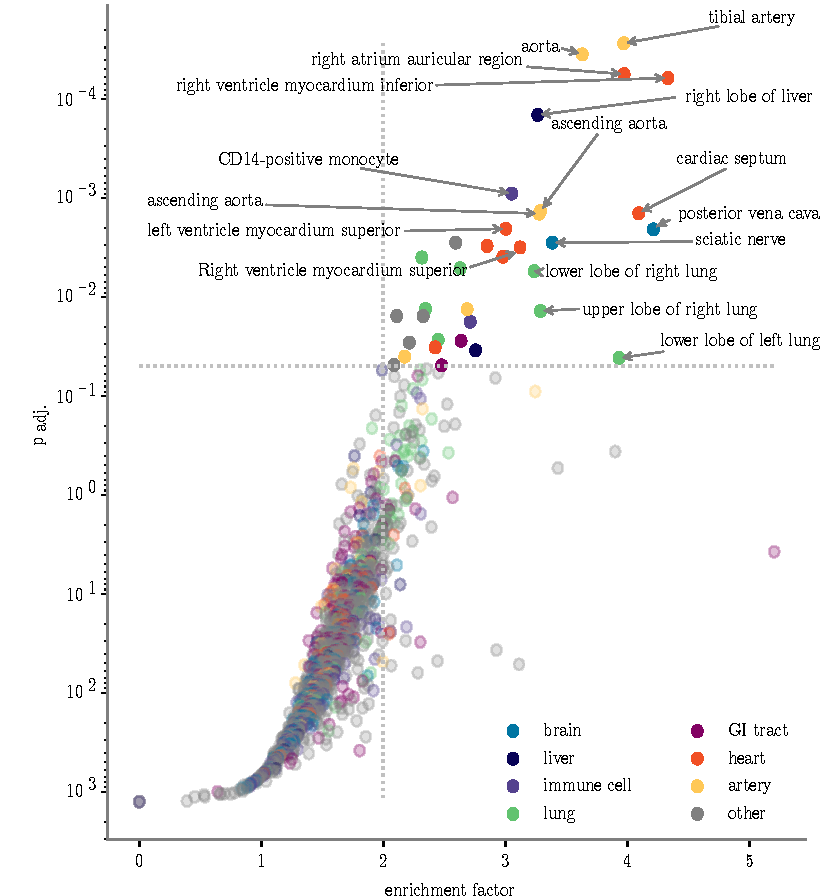
\includegraphics{Abbildung/enrichment_scatter.pdf}

	\begin{minipage}{\captionwidth}
		\caption[enrichemtn]{\uzlemph{Enrichment Analysis} \newline This stuff actually seems to be working!!}
		\label{fig:enrichment}
	\end{minipage}
\end{figure}

As seen in figure \ref{fig:enrichment}, statistical signifcant enrichment ($p_{adj.}<0.05$) was observed for 34 biosamples. These biosamples were annoted using Cellosaurus data. The most prominent groups of associated tissues were heart (8), lung (7) and artery (6).


\begin{table}[h!]
\capstart
\centering
\begin{minipage}{\captionwidth}
    \caption[enriched tissues]{\uzlemph{Enriched tissues}}
    \label{tab:enriched_tissues}
\end{minipage}
\begin{tabular}{|c|c|}
    \hline
    tissue      & count in significant biosamples \\ \hline
    heart       & 8                               \\
    lung        & 7                               \\
    artery      & 6                               \\
    liver       & 2                               \\
    GI tract    & 2                               \\
    brain       & 2                               \\
    immune cell & 2                               \\
    other       & 5                               \\ \hline
    total       & 34                              \\ \hline
    \end{tabular}
\end{table}
